% figure1_workflow.tex — Cross-Layer Security Verification Workflow (Figure 1)
% Standalone compilable document: pdflatex figure1_workflow.tex
\documentclass[border=6pt]{standalone}

\usepackage[T1]{fontenc}
\usepackage{lmodern}
\usepackage{tikz}
\usepackage{amsmath,amssymb}
\usetikzlibrary{
  positioning,
  shapes.geometric,
  arrows.meta,
  backgrounds,
  fit,
  calc
}

% ── Colour palette ──────────────────────────────────────────────────
\definecolor{inputBlue}{HTML}{3B82F6}
\definecolor{threatRed}{HTML}{DC2626}
\definecolor{pipelinePurple}{HTML}{7C3AED}
\definecolor{checkYellow}{HTML}{EAB308}
\definecolor{passGreen}{HTML}{16A34A}
\definecolor{softOrange}{HTML}{EA580C}
\definecolor{hardRed}{HTML}{B91C1C}
\definecolor{dashPurple}{HTML}{DDD6FE}

% ── Node styles ─────────────────────────────────────────────────────
\tikzset{
  base/.style={
    draw, rounded corners=3pt, minimum height=10mm,
    text width=26mm, align=center, font=\sffamily\scriptsize,
    line width=0.6pt
  },
  inputNode/.style={
    base, fill=inputBlue!12, draw=inputBlue, text=inputBlue!90!black
  },
  threatNode/.style={
    base, fill=threatRed!10, draw=threatRed,
    text=threatRed!90!black, text width=34mm, minimum height=16mm
  },
  pipeNode/.style={
    base, fill=pipelinePurple!10, draw=pipelinePurple,
    text=pipelinePurple!90!black, text width=24mm
  },
  checkNode/.style={
    draw, diamond, aspect=2.4, inner sep=1pt,
    fill=checkYellow!18, draw=checkYellow!80!black,
    text=checkYellow!90!black, font=\sffamily\scriptsize,
    align=center, line width=0.6pt, text width=28mm
  },
  verdictPass/.style={
    base, fill=passGreen!12, draw=passGreen,
    text=passGreen!90!black, text width=22mm
  },
  verdictSoft/.style={
    base, fill=softOrange!12, draw=softOrange,
    text=softOrange!90!black, text width=22mm
  },
  verdictHard/.style={
    base, fill=hardRed!12, draw=hardRed,
    text=hardRed!90!black, text width=22mm
  },
  every edge/.style={
    draw, -{Stealth[length=5pt,width=4pt]}, line width=0.55pt,
    color=black!65
  },
  groupBox/.style={
    draw=pipelinePurple!60, dashed, rounded corners=5pt,
    inner sep=5pt, fill=dashPurple!25, line width=0.7pt
  }
}

\begin{document}
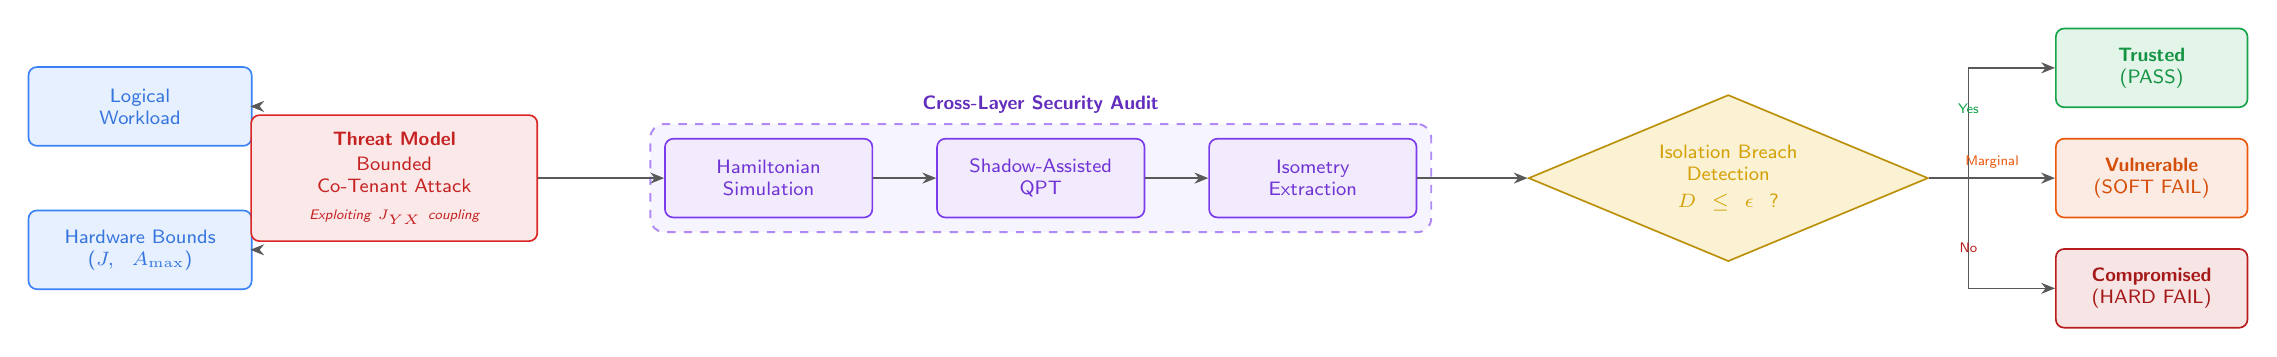
\begin{tikzpicture}[node distance=10mm and 12mm]

% ── STAGE 1: Inputs ────────────────────────────────────────────────
\node[inputNode] (A) {Logical\\Workload};
\node[inputNode, below=8mm of A] (B) {Hardware Bounds\\($J,\; A_{\max}$)};

% ── STAGE 2: Threat Model ──────────────────────────────────────────
\node[threatNode, right=14mm of $(A)!0.5!(B)$] (C) {
  \textbf{Threat Model}\\[1pt]
  Bounded\\Co-Tenant Attack\\[2pt]
  {\tiny\itshape Exploiting $J_{YX}$ coupling}
};

% ── STAGE 3: Cross-Layer Pipeline ──────────────────────────────────
\node[pipeNode, right=16mm of C] (D1) {Hamiltonian\\Simulation};
\node[pipeNode, right=8mm of D1]  (D2) {Shadow-Assisted\\QPT};
\node[pipeNode, right=8mm of D2]  (D3) {Isometry\\Extraction};

% Dashed group box around pipeline
\begin{scope}[on background layer]
  \node[groupBox, fit=(D1)(D2)(D3),
        label={[font=\sffamily\scriptsize\bfseries,
                text=pipelinePurple!80!black]
               above:Cross-Layer Security Audit}] (Dbox) {};
\end{scope}

% ── STAGE 4: Security Check ────────────────────────────────────────
\node[checkNode, right=14mm of D3] (E) {
  Isolation Breach\\Detection\\[2pt]
  $D \le \epsilon\;$?
};

% ── STAGE 5: Verdicts ──────────────────────────────────────────────
\node[verdictPass, right=16mm of E, yshift=14mm]  (F1)
  {\textbf{Trusted}\\(PASS)};
\node[verdictSoft, right=16mm of E]               (F2)
  {\textbf{Vulnerable}\\(SOFT FAIL)};
\node[verdictHard, right=16mm of E, yshift=-14mm] (F3)
  {\textbf{Compromised}\\(HARD FAIL)};

% ── EDGES ───────────────────────────────────────────────────────────
% Inputs → Threat Model
\draw[every edge] (A.east) -- (C.west |- A.east);
\draw[every edge] (B.east) -- (C.west |- B.east);

% Threat Model → Pipeline
\draw[every edge] (C.east) -- (D1.west);

% Pipeline internal
\draw[every edge] (D1.east) -- (D2.west);
\draw[every edge] (D2.east) -- (D3.west);

% Pipeline → Check
\draw[every edge] (D3.east) -- (E.west);

% Check → Verdicts
\draw[every edge] (E.east) -- ++(5mm,0) |- (F1.west)
  node[pos=0.25, above, font=\sffamily\tiny, text=passGreen]{Yes};
\draw[every edge] (E.east) -- (F2.west)
  node[midway, above, font=\sffamily\tiny, text=softOrange]{Marginal};
\draw[every edge] (E.east) -- ++(5mm,0) |- (F3.west)
  node[pos=0.25, below, font=\sffamily\tiny, text=hardRed]{No};

\end{tikzpicture}
\end{document}
